
\section{Classical Methods of Pseudorandom Number Generation}

Classical pseudorandom number generators are based on simple mathematical constructions, typically involving modular arithmetic and linear recurrence relations. Despite their simplicity, they form the basis for many modern designs and provide important insight into the structure of deterministic random-like sequences.

In this section, we present three fundamental classes of classical generators: the Linear Congruential Generator (LCG), the Lehmer generator, and combined generators.

\subsection{Linear Congruential Generator (LCG)}

The Linear Congruential Generator is one of the simplest and most widely studied pseudorandom number generators~\cite{hull1962random,knuth1997art}. It is defined by the recurrence relation:

\[
x_{n+1} = (a x_n + c) \bmod m,
\]

where:
\begin{itemize}
    \item $x_n$ is the current state,
    \item $a$ is the multiplier,
    \item $c$ is the increment,
    \item $m$ is the modulus,
    \item $x_0$ is the seed.
\end{itemize}

The state space of an LCG is the finite ring $\mathbb{Z}_m$, and thus all values satisfy $x_n \in \{0,1,\dots,m-1\}$.

\subsubsection{Period of LCG}

The maximum possible period of an LCG is $m$. This full period is achieved if and only if the following conditions hold:

\begin{itemize}
    \item $\gcd(c, m) = 1$,
    \item $a - 1$ is divisible by all prime factors of $m$,
    \item if $m$ is divisible by $4$, then $a - 1$ is also divisible by $4$.
\end{itemize}

These conditions are known as the Hull--Dobell theorem, which characterizes full-period LCGs~\cite{hull1962random}.

\subsubsection{Properties and Limitations}

LCGs are computationally efficient and easy to implement. However, their statistical quality depends strongly on the choice of parameters.

A well-known drawback is that sequences generated by LCGs exhibit lattice structure when considered in higher dimensions. This geometric regularity reduces their suitability for high-dimensional simulations such as Monte Carlo methods.

Additionally, the period may be significantly smaller than $m$ if parameters are poorly chosen.

\subsubsection{Example of LCG}

Example with parameters $m = 9$, $a = 2$, $c = 1$, $x_0 = 1$:

\begin{table}[htbp]
\centering
\small
\begin{tabular}{|c|c|}
\hline
$n$ & $x_n$ \\
\hline
0 & 1 \\
1 & 3 \\
2 & 7 \\
3 & 6 \\
4 & 4 \\
5 & 0 \\
6 & 1 \\
\hline
\end{tabular}
\caption{Example sequence generated by an LCG}
\end{table}

\subsubsection{C++ Implementation}

The theoretical recurrence relation of the Linear Congruential Generator can be translated directly into C++. The internal state of the generator is stored as an unsigned integer, while the parameters $a$, $c$, and $m$ are represented respectively by the multiplier, increment, and modulus.

The method \texttt{next()} applies the recurrence

\[
x_{n+1} = (a x_n + c) \bmod m
\]

and returns the newly computed state.

\cppfile[
    caption={Core \texttt{next()} function of the Linear Congruential Generator},
    label={lst:lcg-next}
]{codes/lcg/lcg_next.cpp}

The implementation is a direct translation of the mathematical formula. First, the current state is multiplied by the multiplier $a$, then the increment $c$ is added, and finally the result is reduced modulo $m$. The new value becomes the next internal state and is returned as the output of the generator. The use of \texttt{\_\_uint128\_t} prevents overflow during the intermediate multiplication before the modulo operation is applied.

\subsubsection{Experimental Comparison}

To illustrate the influence of parameters, three LCG variants were compared. The first generator uses parameters satisfying the Hull--Dobell conditions. The second generator uses a large modulus but poorly chosen parameters. The third generator differs from the good one only by one parameter: the increment is even, so the condition $\gcd(c,m)=1$ is violated.

\begin{table}[htbp]
\centering
\small
\resizebox{\textwidth}{!}{%
\begin{tabular}{|l|r|r|r|}
\hline
Parameter & Good LCG & Bad large-range LCG & One broken condition \\
\hline
Seed & $123456789$ & $123456789$ & $123456789$ \\
Multiplier $a$ & $1103515245$ & $65539$ & $1103515245$ \\
Increment $c$ & $12345$ & $0$ & $12344$ \\
Modulus $m$ & $2^{31}$ & $2^{31}$ & $2^{31}$ \\
\hline
\end{tabular}%
}
\caption{LCG parameter sets used in the experiment}
\label{tab:lcg-parameters}
\end{table}

For each generator, $100000$ generated values were used to compute basic statistics. The histogram was divided into $20$ buckets. The sequence plot and the successive-value plot were generated using $5000$ values.

\begin{table}[htbp]
\centering
\small
\resizebox{\textwidth}{!}{%
\begin{tabular}{|l|r|r|r|}
\hline
Statistic & Good LCG & Bad large-range LCG & One broken condition \\
\hline
Min & $14984$ & $26007$ & $18045$ \\
Max & $2147472790$ & $2147458605$ & $2147483589$ \\
Mean & $1072058253.99$ & $1073741022.56$ & $1072768794.75$ \\
Std. dev. & $618784777.74$ & $619155200.59$ & $618797107.84$ \\
One-bit ratio & $0.499968$ & $0.532329$ & $0.499702$ \\
$\chi^2$ & $17.2004$ & $11.7680$ & $14.9208$ \\
\hline
\end{tabular}%
}
\caption{Basic statistics computed from $100000$ LCG outputs}
\label{tab:lcg-statistics}
\end{table}

The good LCG has a mean close to the middle of the interval $[0,2^{31}-1]$ and a one-bit ratio almost equal to $0.5$. This suggests that, at least in this simple experiment, zeros and ones appear in the binary representation with nearly equal frequency.

The bad large-range LCG shows why simple statistics can be misleading. Its minimum, maximum, mean and standard deviation do not look catastrophic. Even the chi-square value for the histogram is not extremely large. However, the one-bit ratio is equal to $0.532329$, which is visibly shifted away from the ideal value $0.5$. This indicates imbalance at the bit level.

The generator with one broken condition looks relatively close to the good one in these basic statistics. This is important, because it shows that a generator can fail a theoretical condition without immediately looking broken in a short one-dimensional test. The problem is structural: when $\gcd(c,m) \neq 1$, the full period is not guaranteed.

\begin{figure}[htbp]
\centering
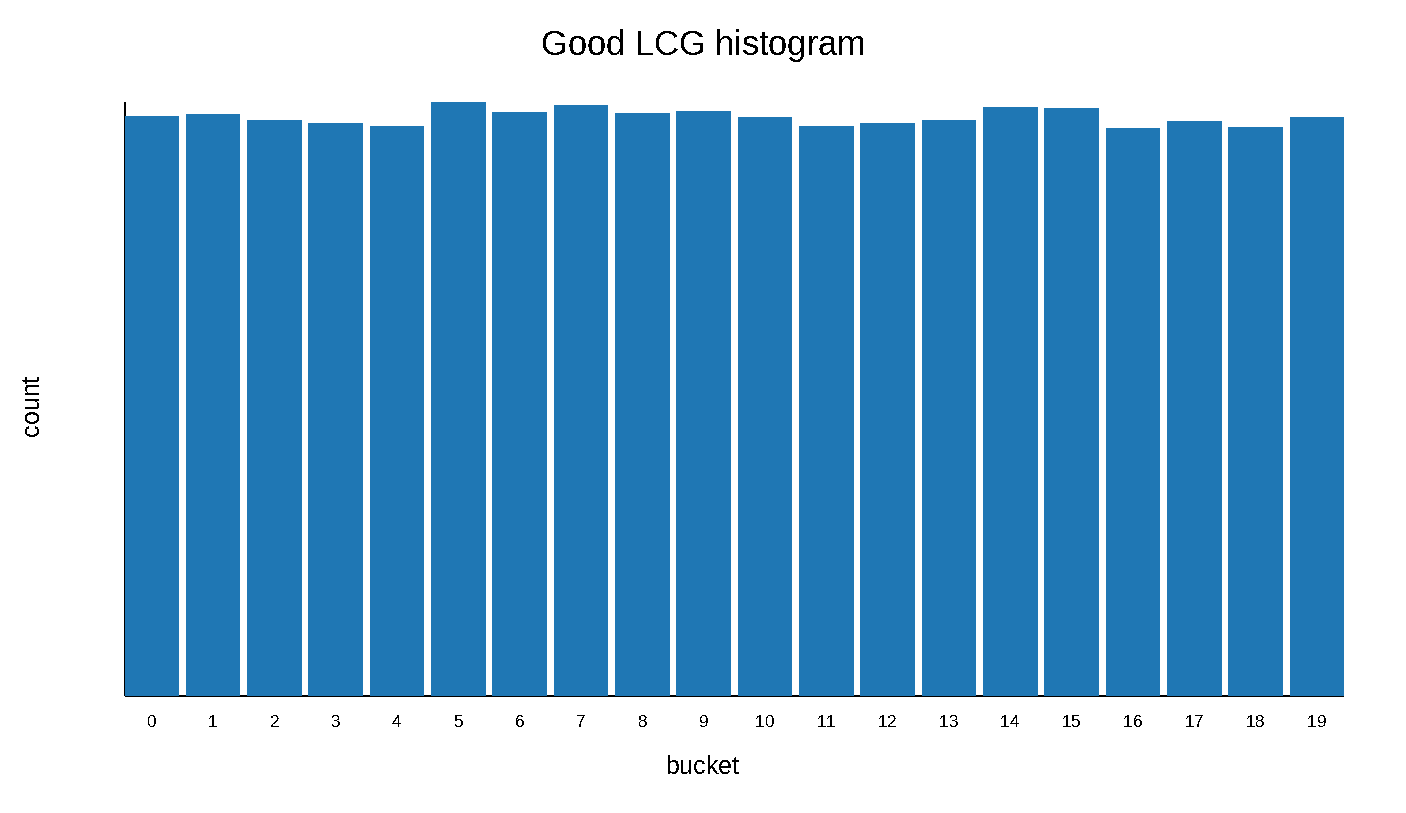
\includegraphics[width=0.48\textwidth]{figures/lcg/good/lcg_good_hull_dobell_31bit_histogram.pdf}
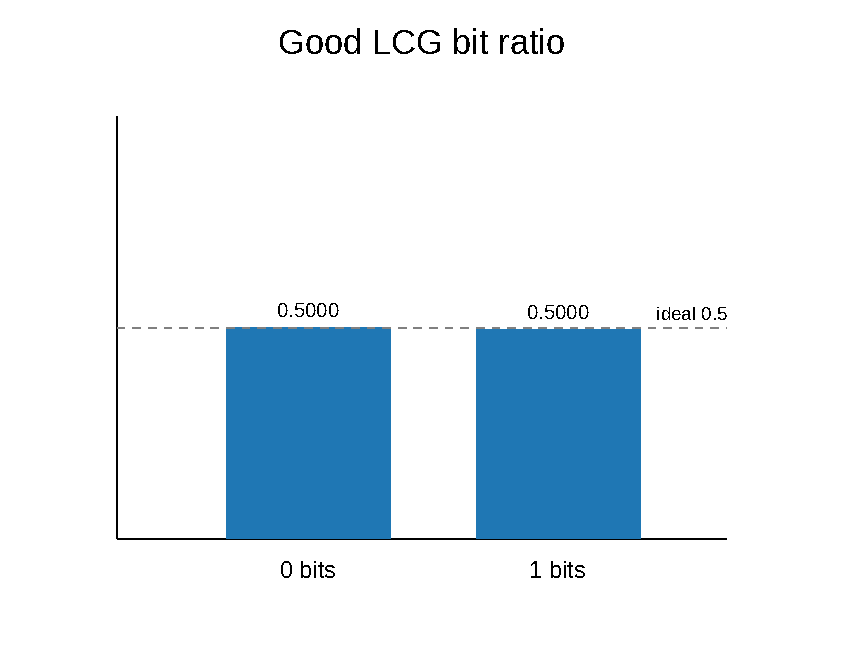
\includegraphics[width=0.48\textwidth]{figures/lcg/good/lcg_good_hull_dobell_31bit_bit_ratio.pdf}
\caption{Histogram and bit ratio for the good LCG}
\label{fig:lcg-good-hist-bits}
\end{figure}

\begin{figure}[htbp]
\centering
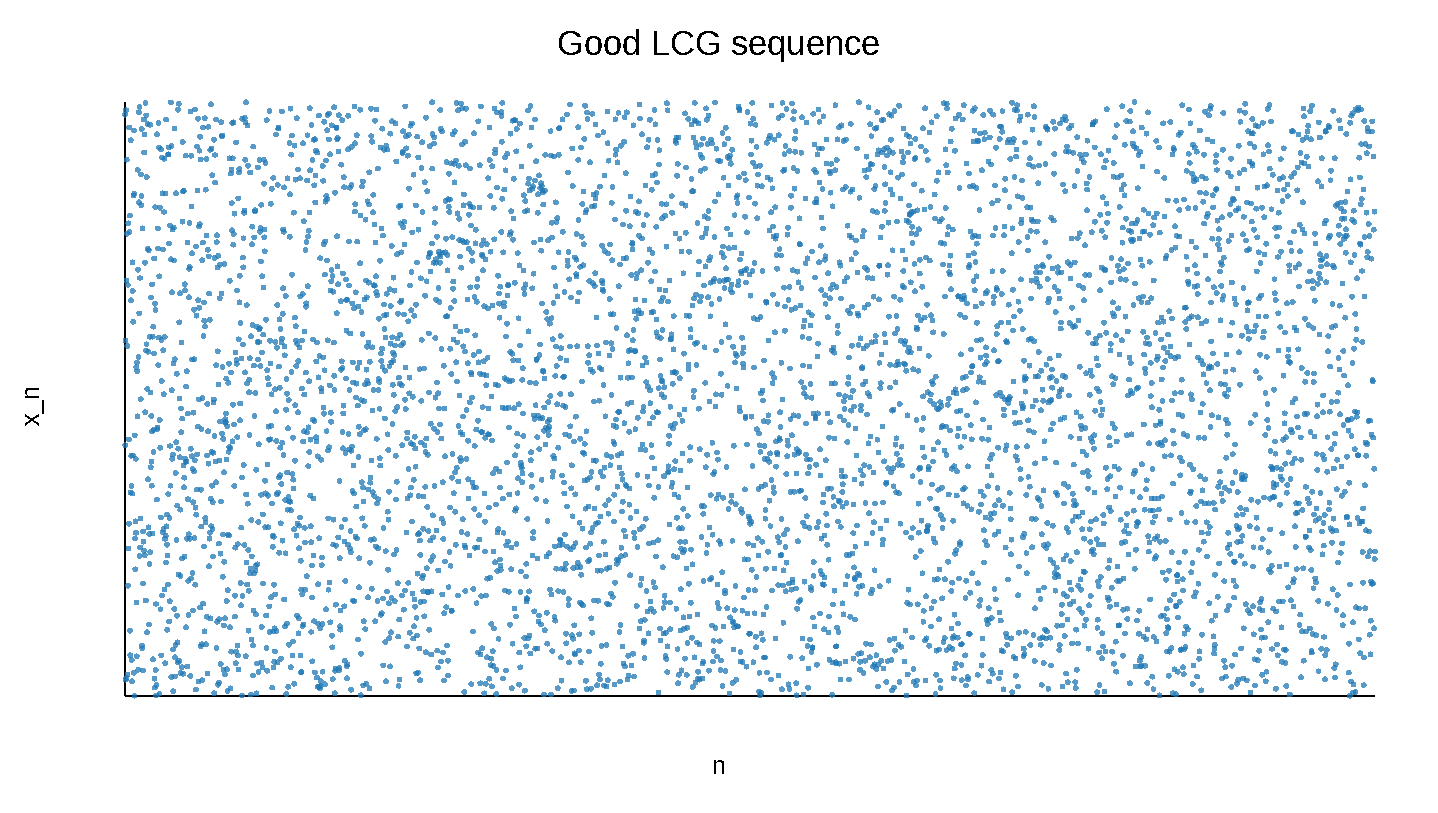
\includegraphics[width=0.48\textwidth]{figures/lcg/good/lcg_good_hull_dobell_31bit_sequence.pdf}
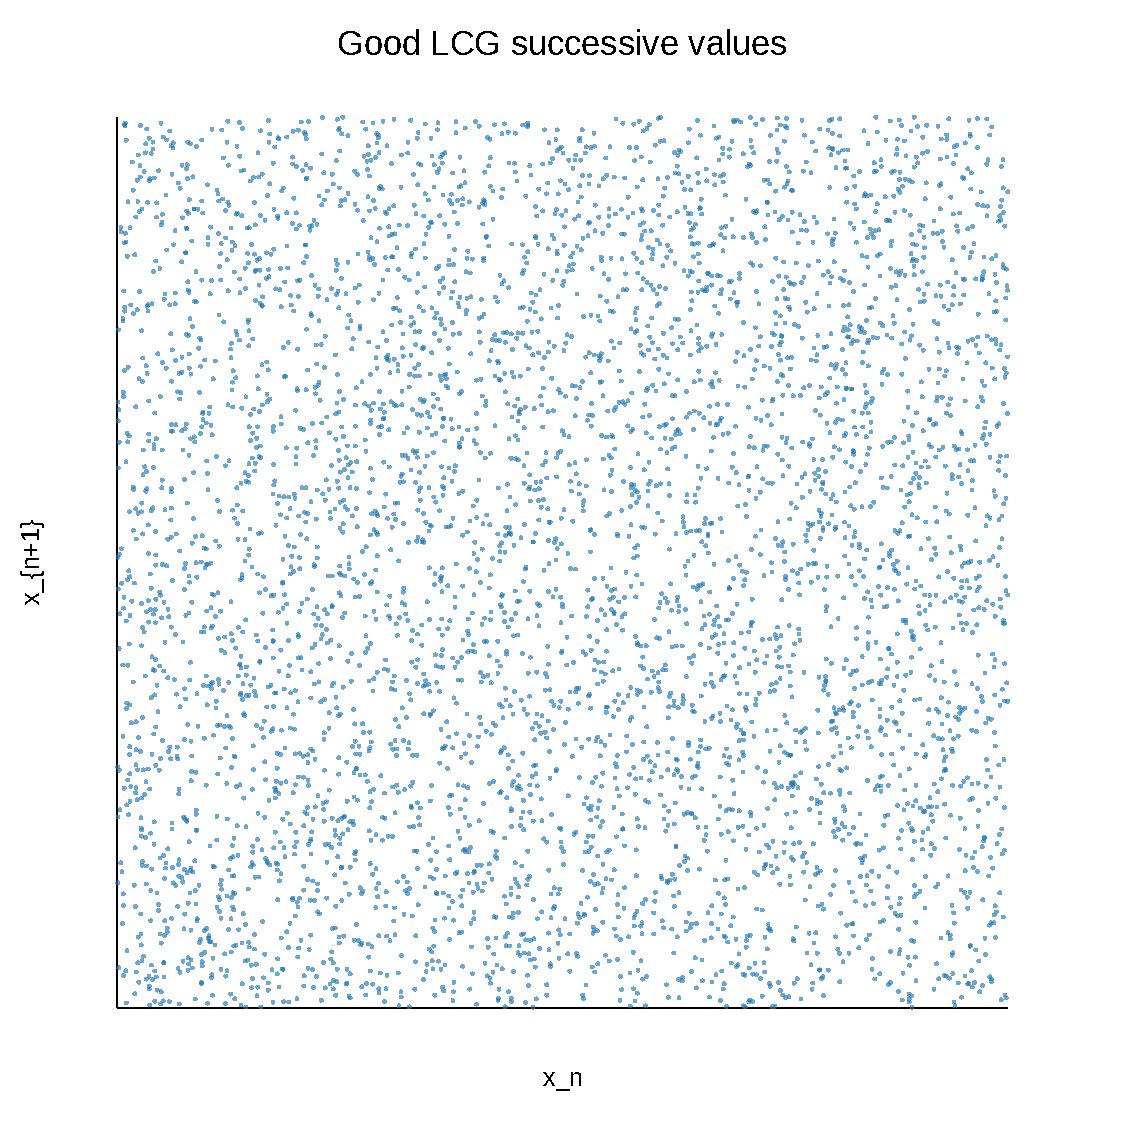
\includegraphics[width=0.48\textwidth]{figures/lcg/good/lcg_good_hull_dobell_31bit_successive_values.pdf}
\caption{Sequence plot and successive-value plot for the good LCG}
\label{fig:lcg-good-seq-succ}
\end{figure}

Figures \ref{fig:lcg-good-hist-bits} and \ref{fig:lcg-good-seq-succ} show that the good LCG covers the output range evenly in this experiment. The histogram is balanced, the bit ratio is close to $0.5$, and the successive-value plot does not collapse into a small visible subset of points.

\begin{figure}[htbp]
\centering
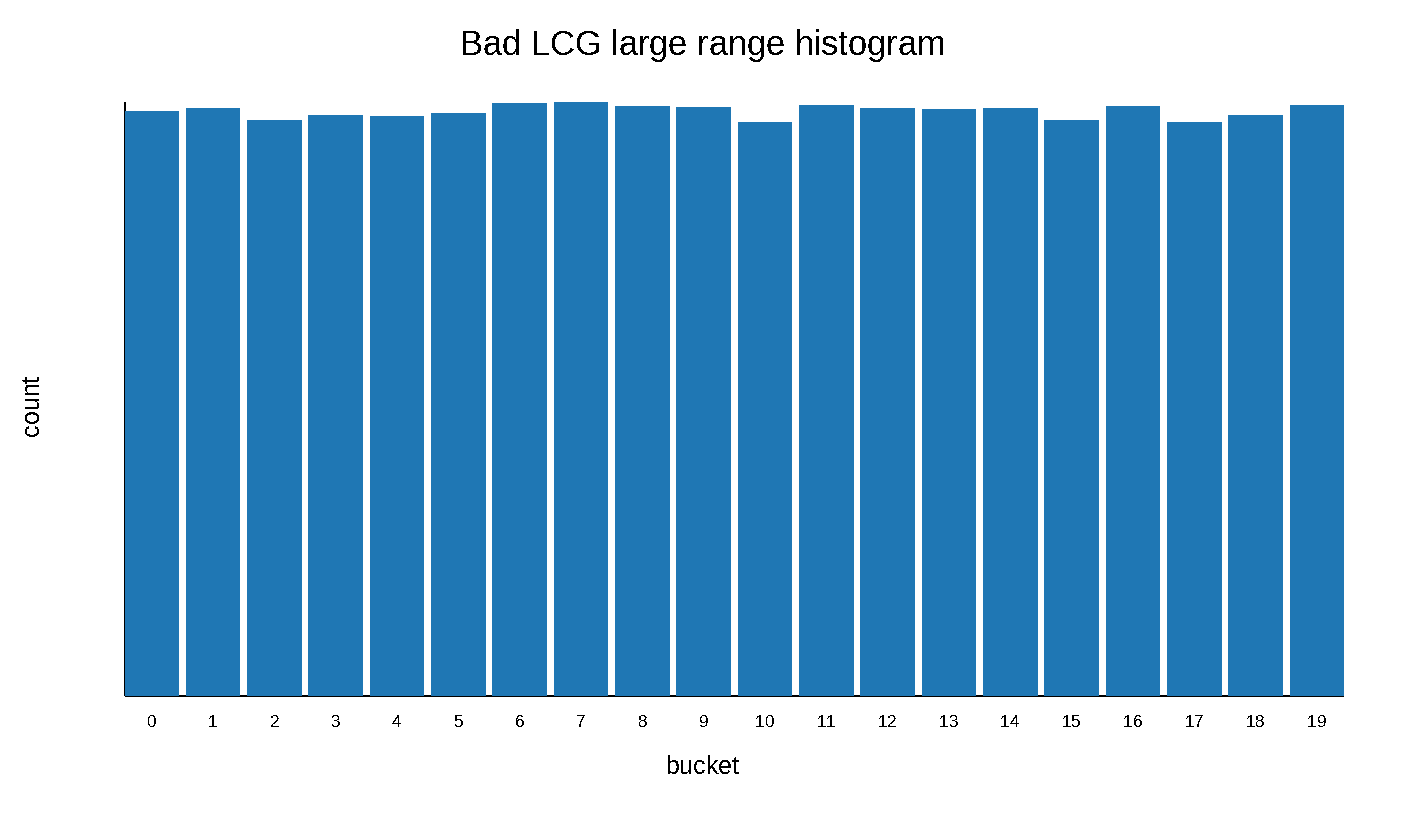
\includegraphics[width=0.48\textwidth]{figures/lcg/bad_large_range/lcg_bad_randu_style_zero_increment_histogram.pdf}
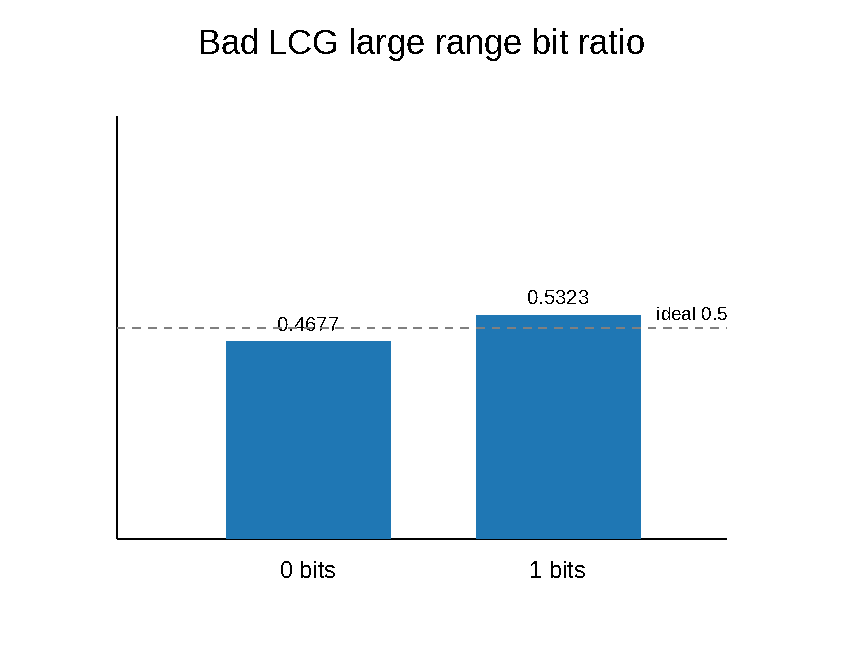
\includegraphics[width=0.48\textwidth]{figures/lcg/bad_large_range/lcg_bad_randu_style_zero_increment_bit_ratio.pdf}
\caption{Histogram and bit ratio for the bad large-range LCG}
\label{fig:lcg-bad-hist-bits}
\end{figure}

\begin{figure}[htbp]
\centering
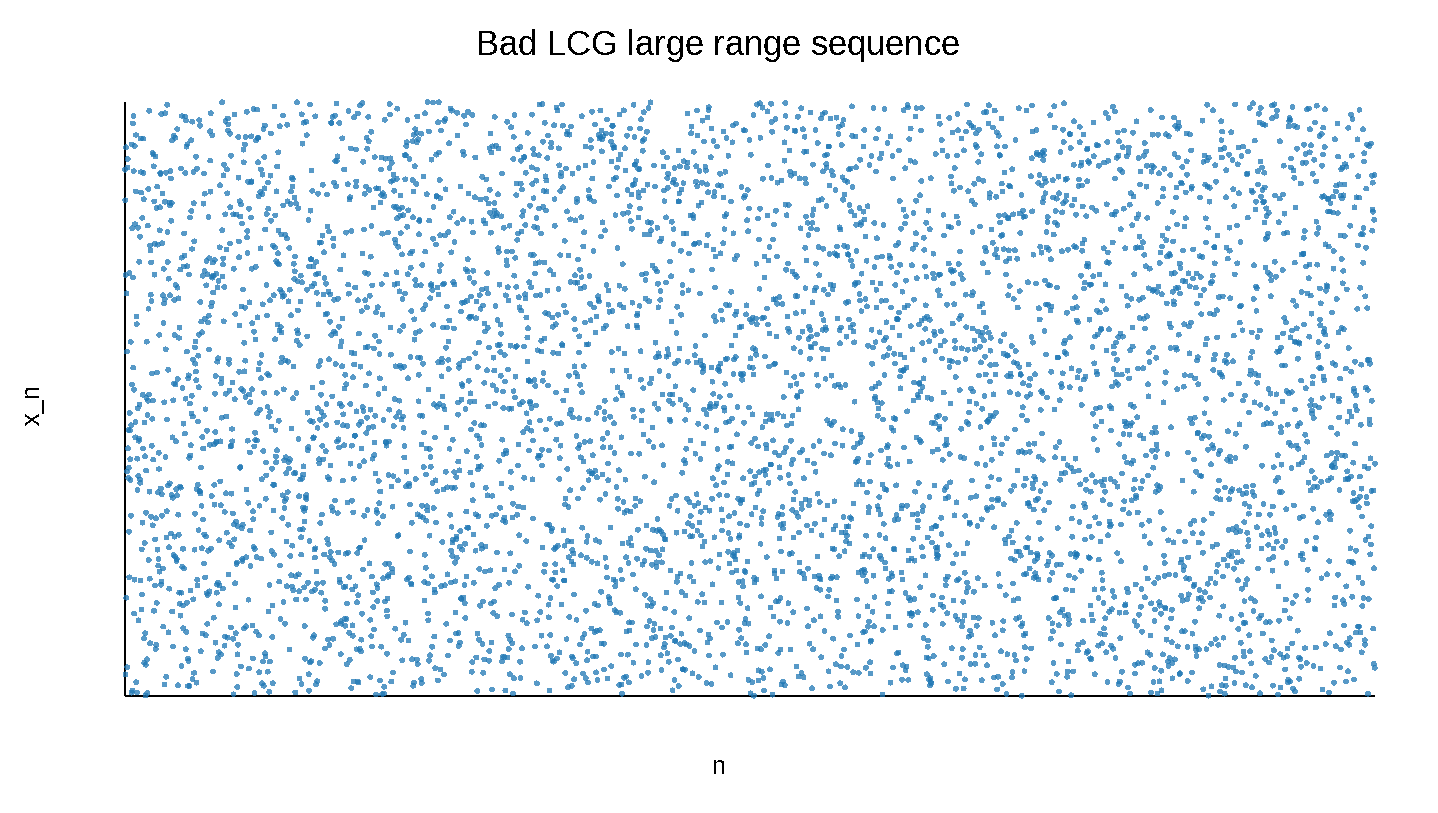
\includegraphics[width=0.48\textwidth]{figures/lcg/bad_large_range/lcg_bad_randu_style_zero_increment_sequence.pdf}
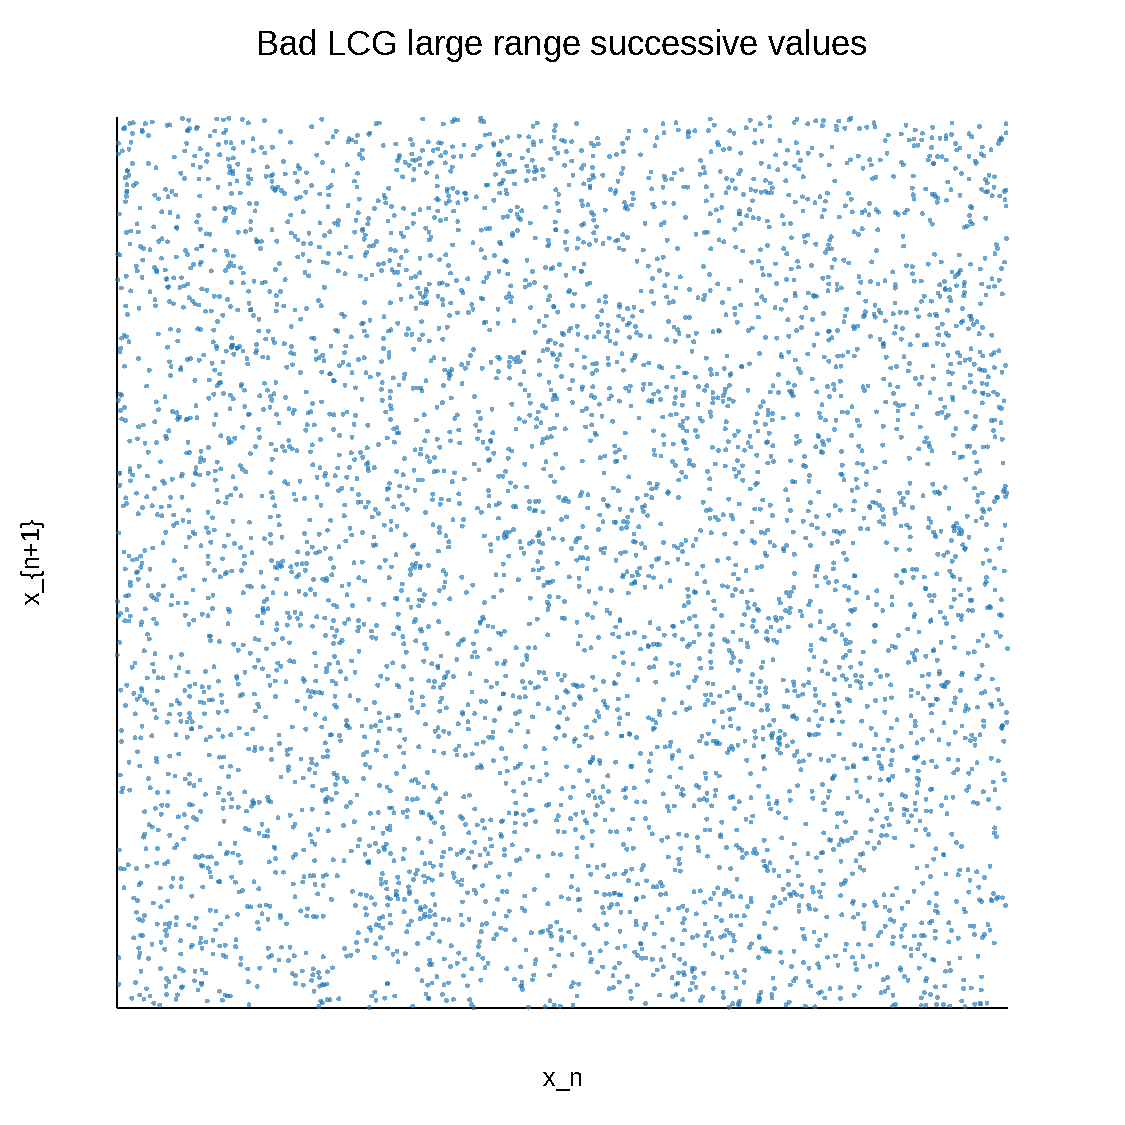
\includegraphics[width=0.48\textwidth]{figures/lcg/bad_large_range/lcg_bad_randu_style_zero_increment_successive_values.pdf}
\caption{Sequence plot and successive-value plot for the bad large-range LCG}
\label{fig:lcg-bad-seq-succ}
\end{figure}

Figures \ref{fig:lcg-bad-hist-bits} and \ref{fig:lcg-bad-seq-succ} show that a large output range alone does not guarantee good randomness. The generator still produces values over a large interval, but the bit-ratio plot reveals a visible bias caused by the poor choice of parameters.

\begin{figure}[htbp]
\centering
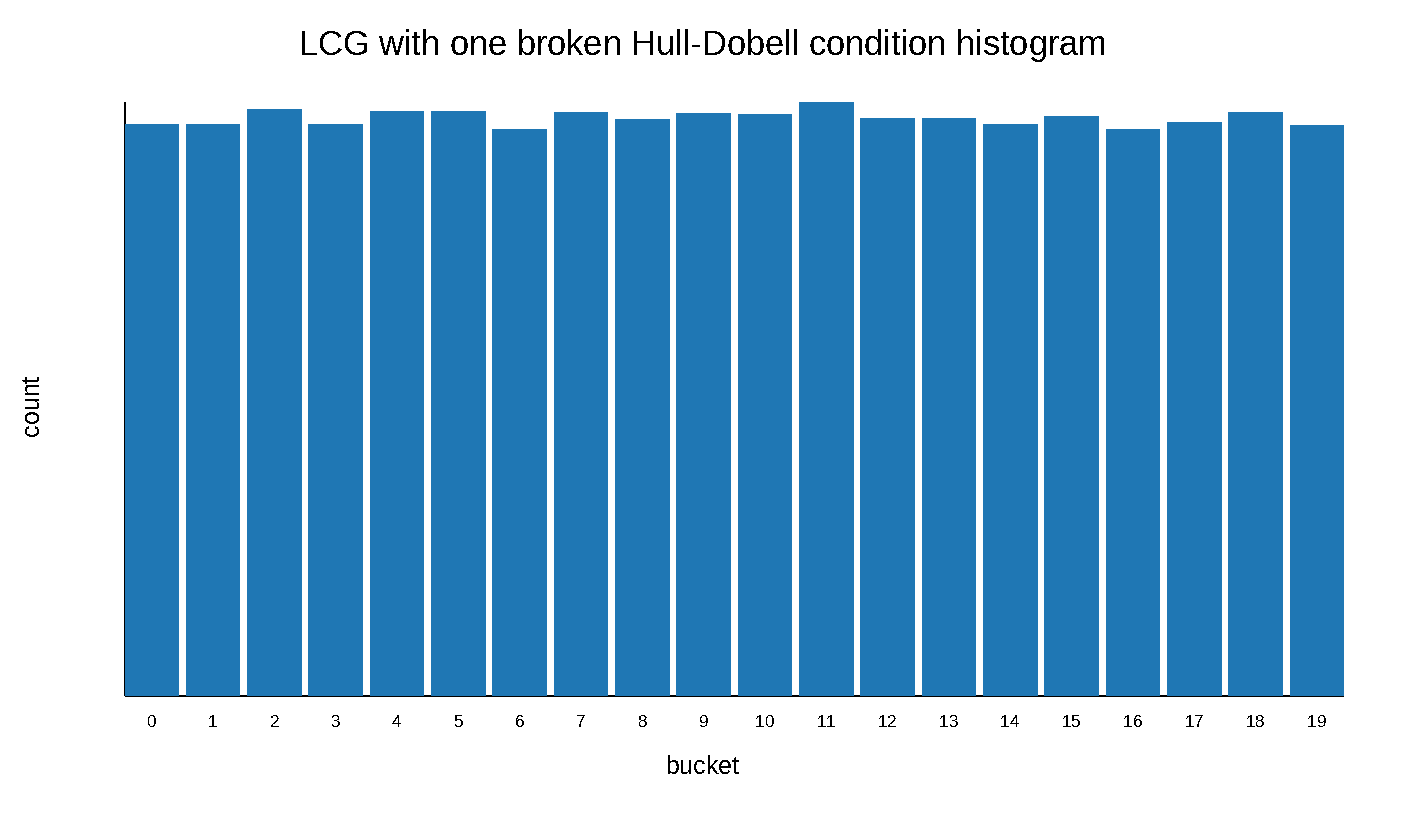
\includegraphics[width=0.48\textwidth]{figures/lcg/single_bad_parameter/lcg_single_bad_even_increment_histogram.pdf}
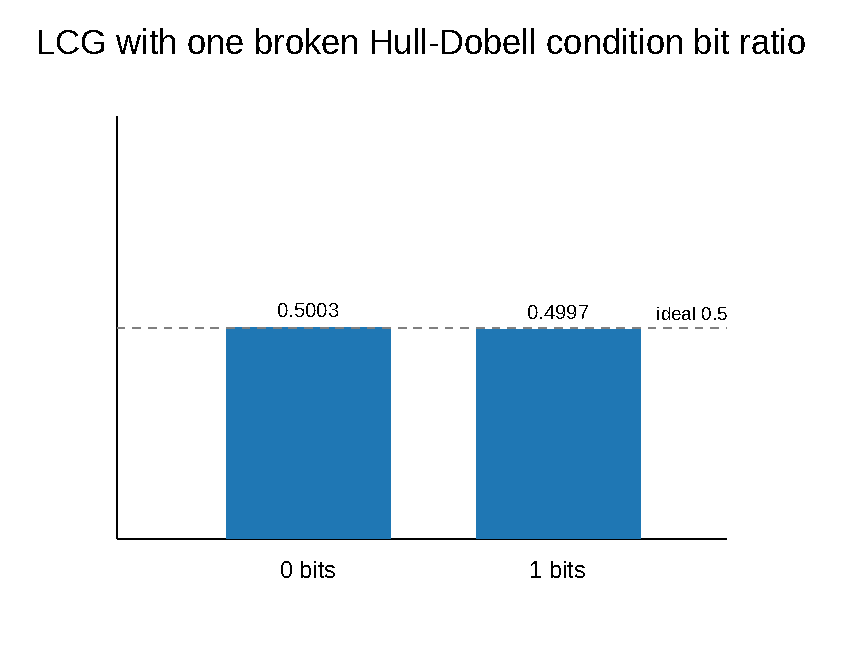
\includegraphics[width=0.48\textwidth]{figures/lcg/single_bad_parameter/lcg_single_bad_even_increment_bit_ratio.pdf}
\caption{Histogram and bit ratio for the LCG with one broken Hull--Dobell condition}
\label{fig:lcg-single-hist-bits}
\end{figure}

\begin{figure}[htbp]
\centering
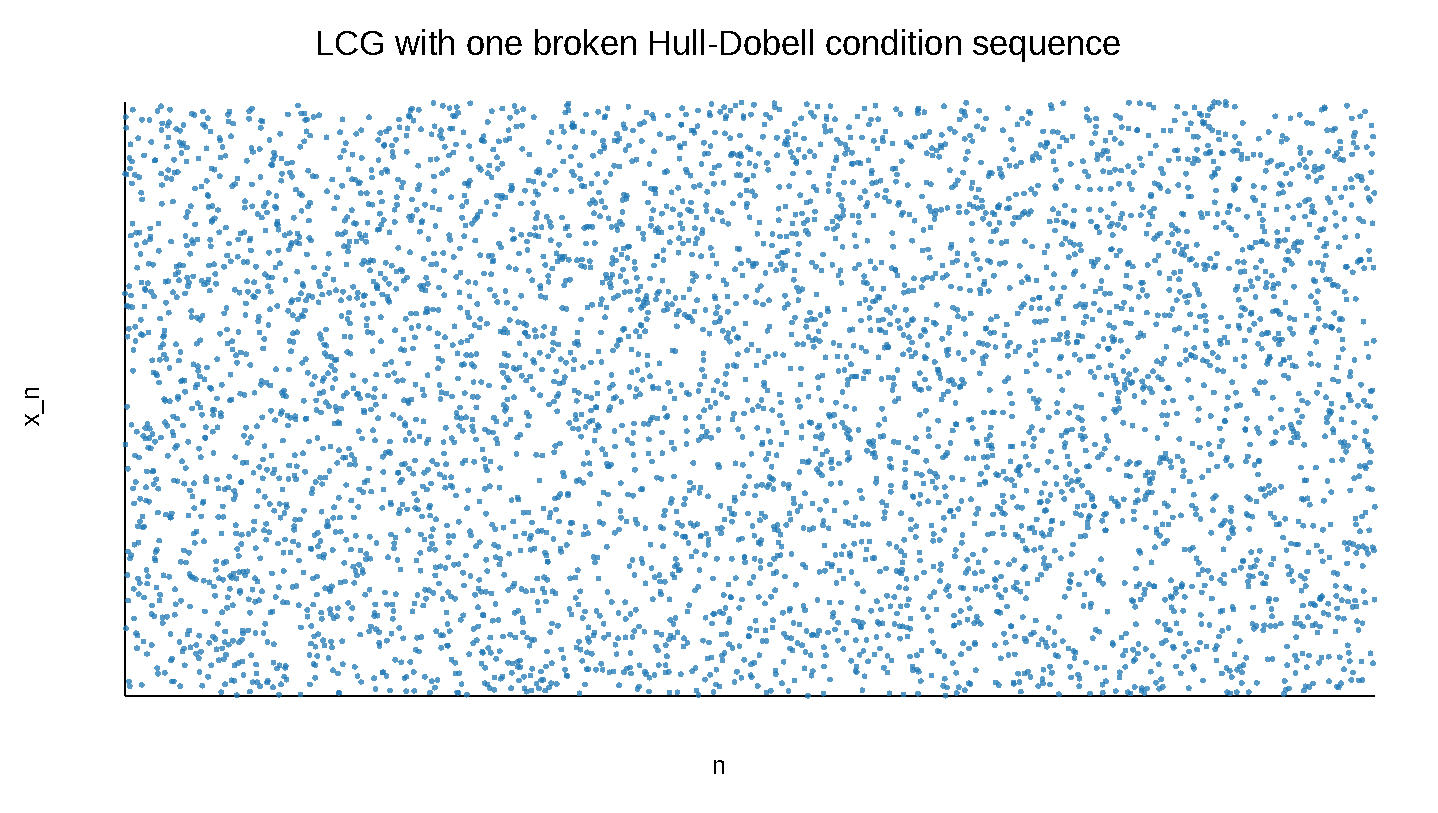
\includegraphics[width=0.48\textwidth]{figures/lcg/single_bad_parameter/lcg_single_bad_even_increment_sequence.pdf}
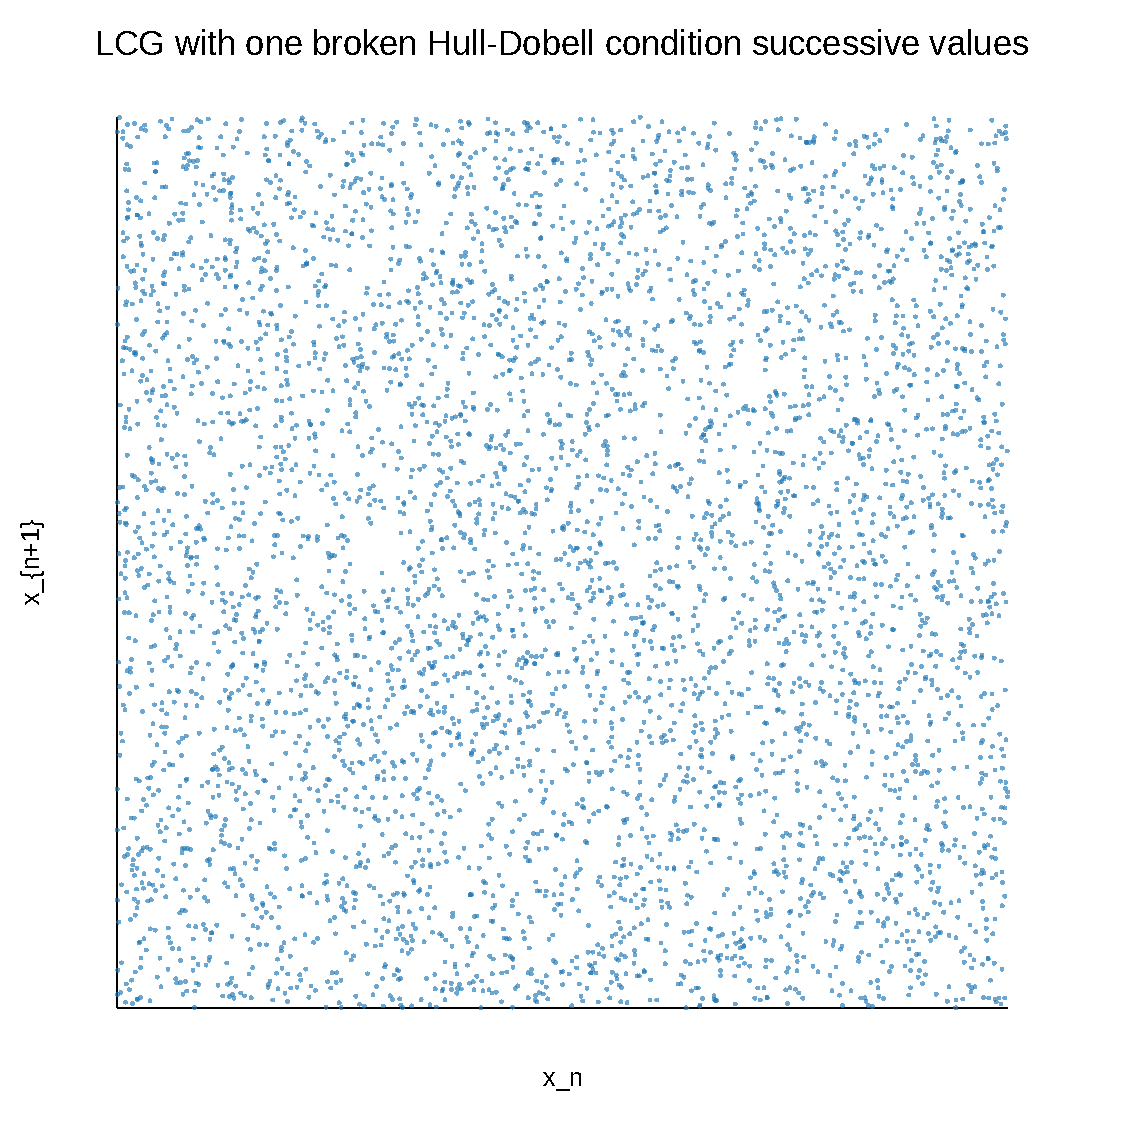
\includegraphics[width=0.48\textwidth]{figures/lcg/single_bad_parameter/lcg_single_bad_even_increment_successive_values.pdf}
\caption{Sequence plot and successive-value plot for the LCG with one broken condition}
\label{fig:lcg-single-seq-succ}
\end{figure}

Figures \ref{fig:lcg-single-hist-bits} and \ref{fig:lcg-single-seq-succ} show that a single broken period condition may still produce visually acceptable plots. This confirms that empirical plots are useful for detecting obvious problems, but they do not replace theoretical period analysis.

\subsection{Lehmer Generator}

The Lehmer generator is a special case of the LCG where the increment $c = 0$~\cite{lehmer1951}. It is defined by:

\[
x_{n+1} = (a x_n) \bmod m.
\]

It is also known as the multiplicative congruential generator.

In this case, the state evolves in the multiplicative group $\mathbb{Z}_m^*$.

\subsubsection{Period}

To achieve a long period, the modulus $m$ is typically chosen as a prime number, and the multiplier $a$ is chosen as a primitive root modulo $m$.

Under these conditions, the generator achieves the maximum period:

\[
T = m - 1.
\]

\subsubsection{Properties}

\begin{itemize}
    \item simpler structure compared to full LCG,
    \item good statistical properties for appropriate parameter choices,
    \item still vulnerable to correlation effects and structural artifacts.
\end{itemize}

\subsubsection{C++ Implementation}

The Lehmer generator uses the same modular idea as LCG, but without an additive increment. Therefore, the transition consists only of multiplication followed by reduction modulo $m$.

\cppfile[
    caption={Core \texttt{next()} function of the Lehmer generator},
    label={lst:lehmer-next}
]{codes/lehmer/lehmer_next.cpp}

The implementation multiplies the current state by the multiplier $a$ and reduces the result modulo $m$. As in the LCG implementation, an extended integer type is used for the intermediate product to avoid overflow before the modulo operation. Since there is no increment, the zero state is absorbing: if the state ever becomes zero, all future values are also zero. For this reason, Lehmer generators are usually analyzed on the non-zero residues modulo $m$.

\subsubsection{Experimental Comparison}

Three Lehmer variants were compared. The good variant uses the classical MINSTD-style parameters with prime modulus $m=2147483647$ and multiplier $a=48271$, a parameter choice in the family of multiplicative congruential generators studied in numerical simulation literature~\cite{lecuyer1999tables}. The bad large-range variant uses $a=m-1$, which produces a very short cycle alternating between two values. The single-bad-parameter variant keeps the same large prime modulus but uses a non-primitive multiplier, which preserves the large numerical range while damaging the period structure.

\begin{table}[htbp]
\centering
\small
\resizebox{\textwidth}{!}{%
\begin{tabular}{|l|r|r|r|}
\hline
Parameter & Good Lehmer & Bad large-range Lehmer & Non-primitive multiplier \\
\hline
Seed & $123456789$ & $123456789$ & $123456789$ \\
Multiplier $a$ & $48271$ & $2147483646$ & $1073741823$ \\
Modulus $m$ & $2147483647$ & $2147483647$ & $2147483647$ \\
\hline
\end{tabular}%
}
\caption{Lehmer parameter sets used in the experiment}
\label{tab:lehmer-parameters}
\end{table}

\begin{table}[htbp]
\centering
\small
\resizebox{\textwidth}{!}{%
\begin{tabular}{|l|r|r|r|}
\hline
Statistic & Good Lehmer & Bad large-range Lehmer & Non-primitive multiplier \\
\hline
Min & $930$ & $123456789$ & $106782249$ \\
Max & $2147479582$ & $2024026858$ & $2040701398$ \\
Mean & $1074185909.16$ & $1073741823.50$ & $1073746274.59$ \\
Std. dev. & $621925036.58$ & $950285034.50$ & $570682073.19$ \\
One-bit ratio & $0.499607$ & $0.500000$ & $0.500000$ \\
$\chi^2$ & $15.3896$ & $900000.0000$ & $13424.2256$ \\
\hline
\end{tabular}%
}
\caption{Basic statistics computed from $100000$ Lehmer outputs}
\label{tab:lehmer-statistics}
\end{table}

The good Lehmer generator has a balanced bit ratio and a low chi-square value, which suggests a relatively even one-dimensional distribution in this experiment. The bad large-range variant is intentionally deceptive: the values are still large and the bit ratio is exactly balanced, but the chi-square value is enormous. This happens because the sequence alternates between only two values, so almost all histogram buckets remain empty. The non-primitive multiplier variant is less trivial, but the chi-square value is still very large, indicating a serious distribution problem.

\begin{figure}[htbp]
\centering
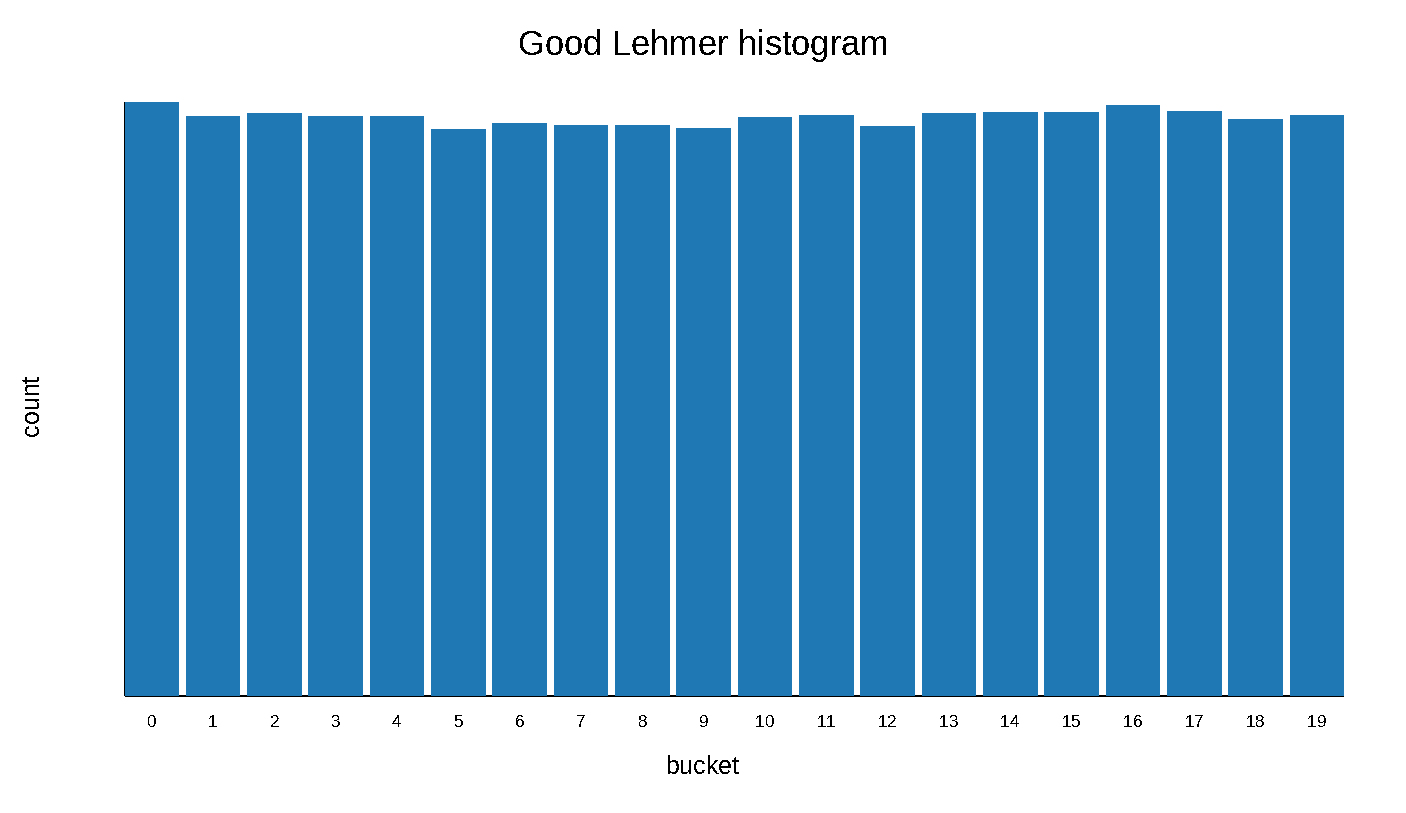
\includegraphics[width=0.48\textwidth]{figures/lehmer/good/lehmer_good_minstd_prime_modulus_histogram.pdf}
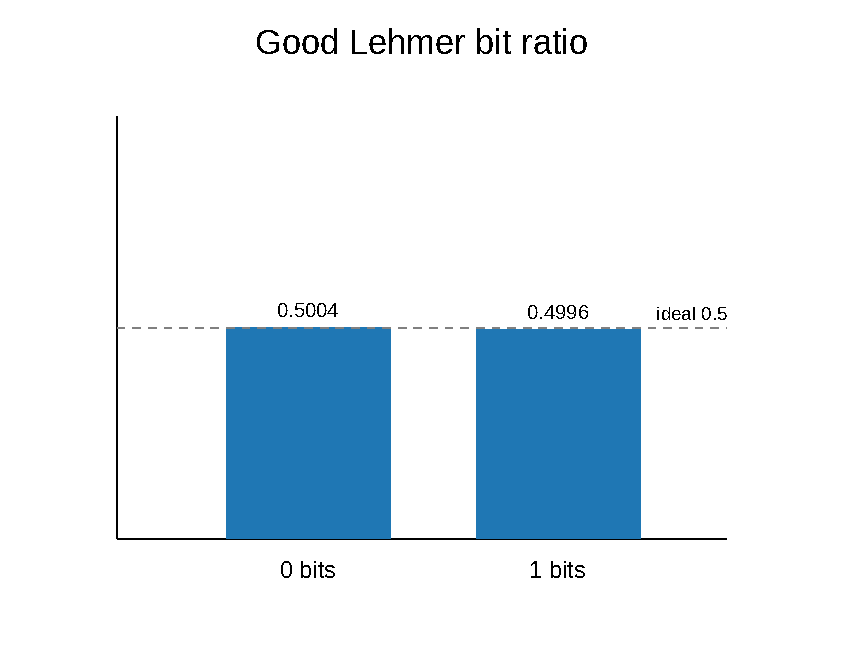
\includegraphics[width=0.48\textwidth]{figures/lehmer/good/lehmer_good_minstd_prime_modulus_bit_ratio.pdf}
\caption{Histogram and bit ratio for the good Lehmer generator}
\label{fig:lehmer-good-hist-bits}
\end{figure}

\begin{figure}[htbp]
\centering
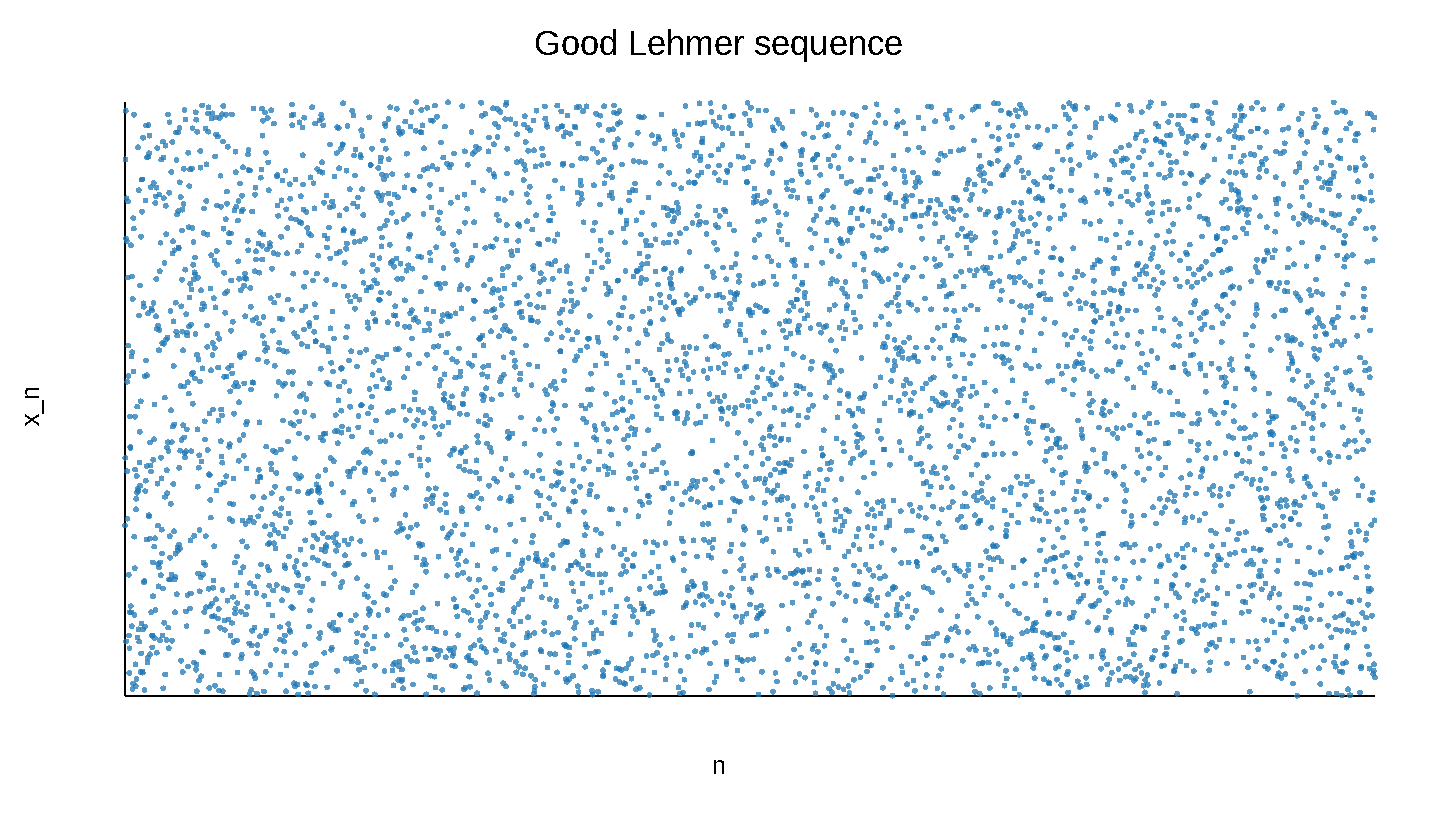
\includegraphics[width=0.48\textwidth]{figures/lehmer/good/lehmer_good_minstd_prime_modulus_sequence.pdf}
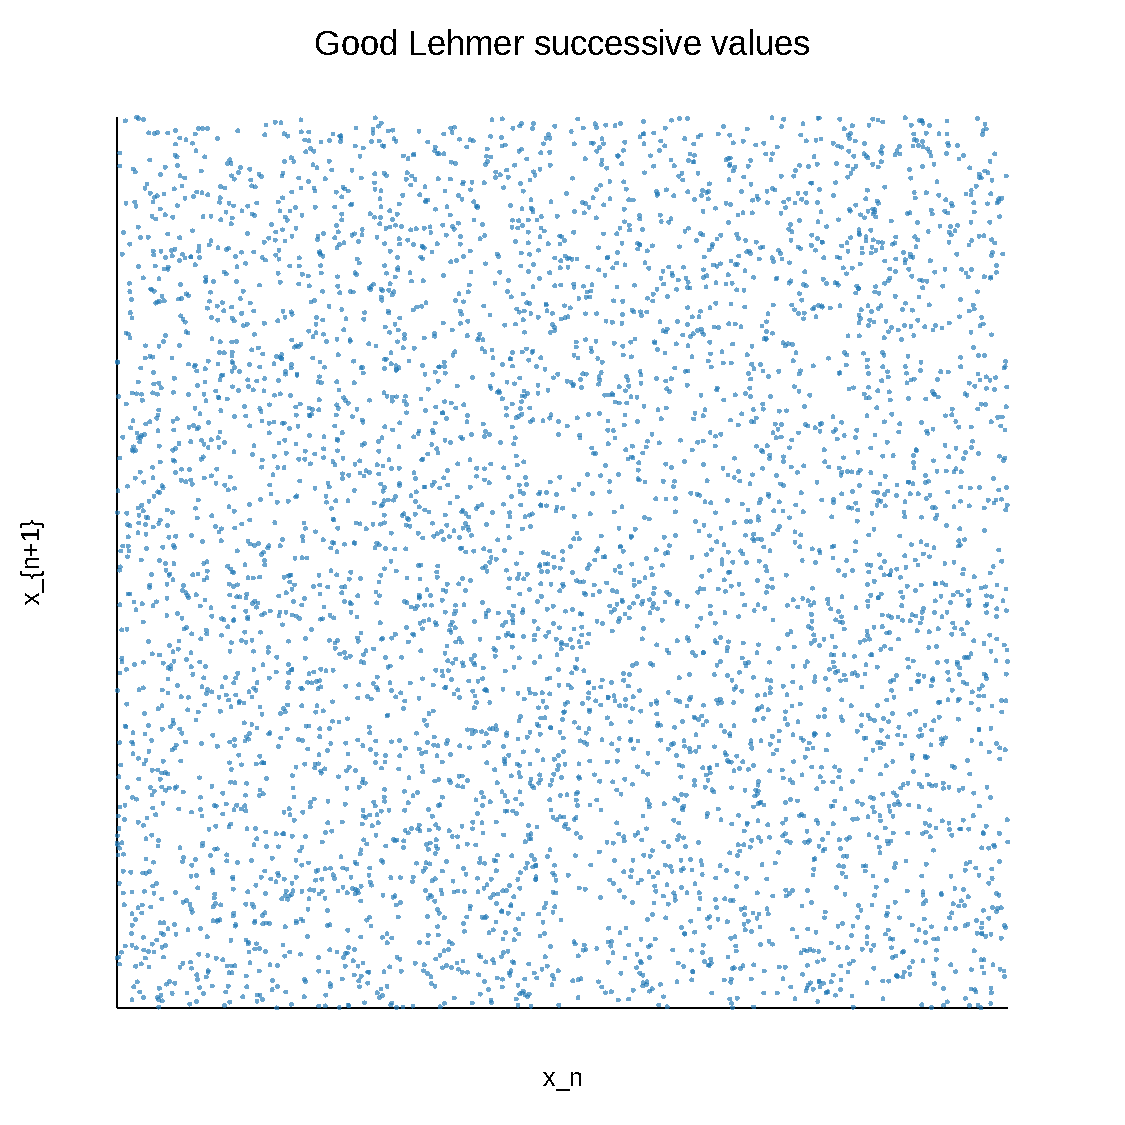
\includegraphics[width=0.48\textwidth]{figures/lehmer/good/lehmer_good_minstd_prime_modulus_successive_values.pdf}
\caption{Sequence plot and successive-value plot for the good Lehmer generator}
\label{fig:lehmer-good-seq-succ}
\end{figure}

Figures \ref{fig:lehmer-good-hist-bits} and \ref{fig:lehmer-good-seq-succ} show that the good Lehmer generator spreads values over the whole interval and keeps the bit ratio close to the ideal value $0.5$.

\begin{figure}[htbp]
\centering
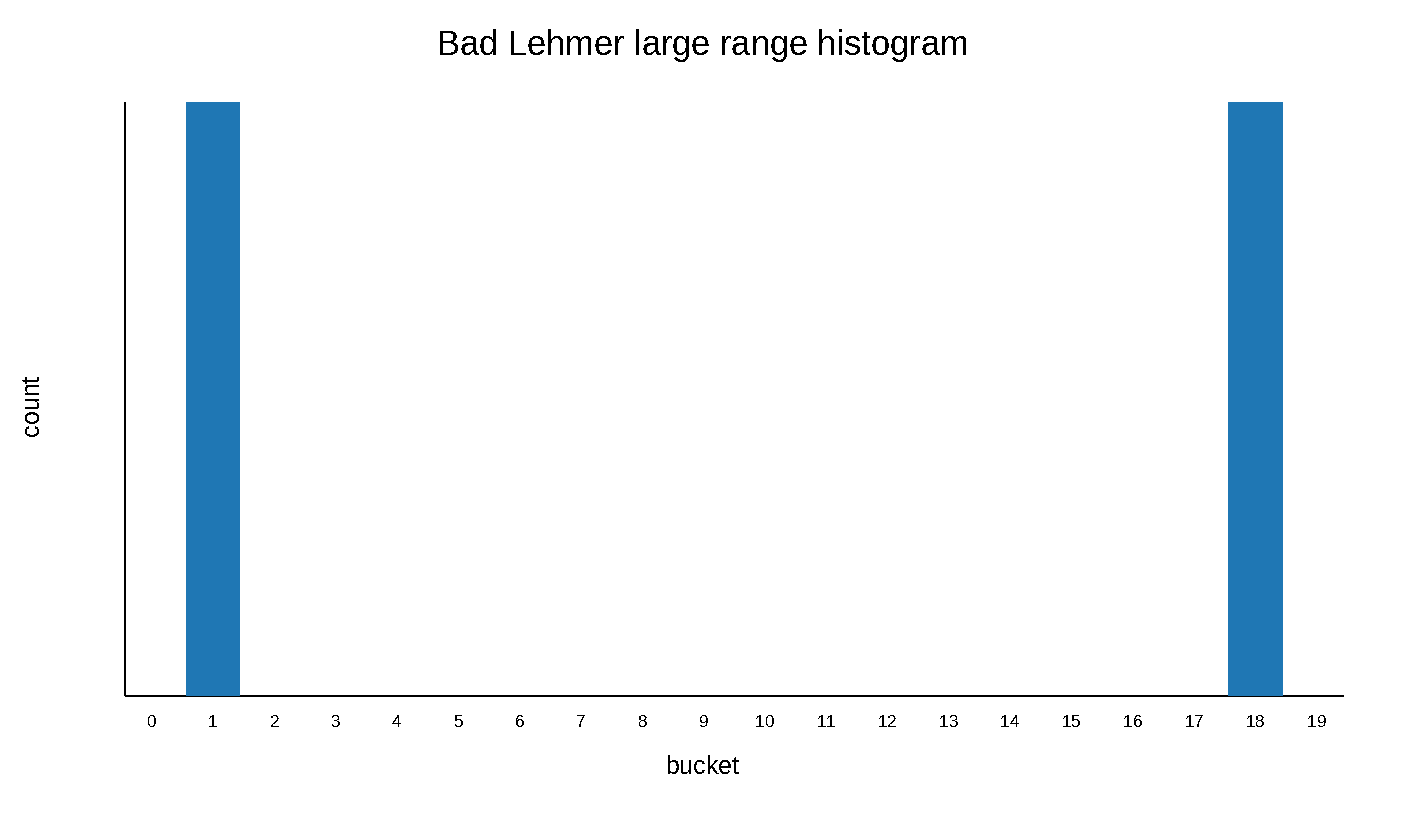
\includegraphics[width=0.48\textwidth]{figures/lehmer/bad_large_range/lehmer_bad_minus_one_multiplier_histogram.pdf}
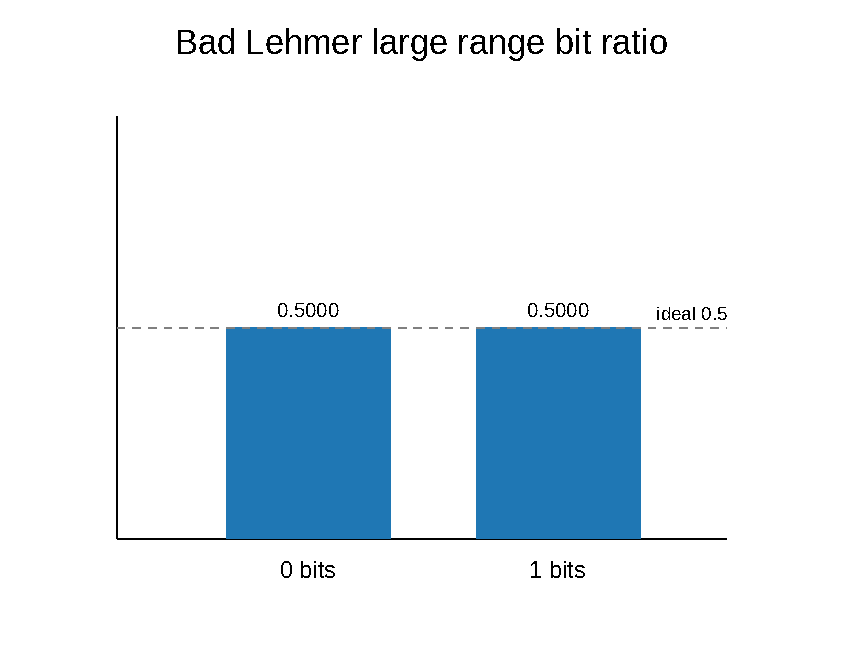
\includegraphics[width=0.48\textwidth]{figures/lehmer/bad_large_range/lehmer_bad_minus_one_multiplier_bit_ratio.pdf}
\caption{Histogram and bit ratio for the bad large-range Lehmer generator}
\label{fig:lehmer-bad-hist-bits}
\end{figure}

\begin{figure}[htbp]
\centering
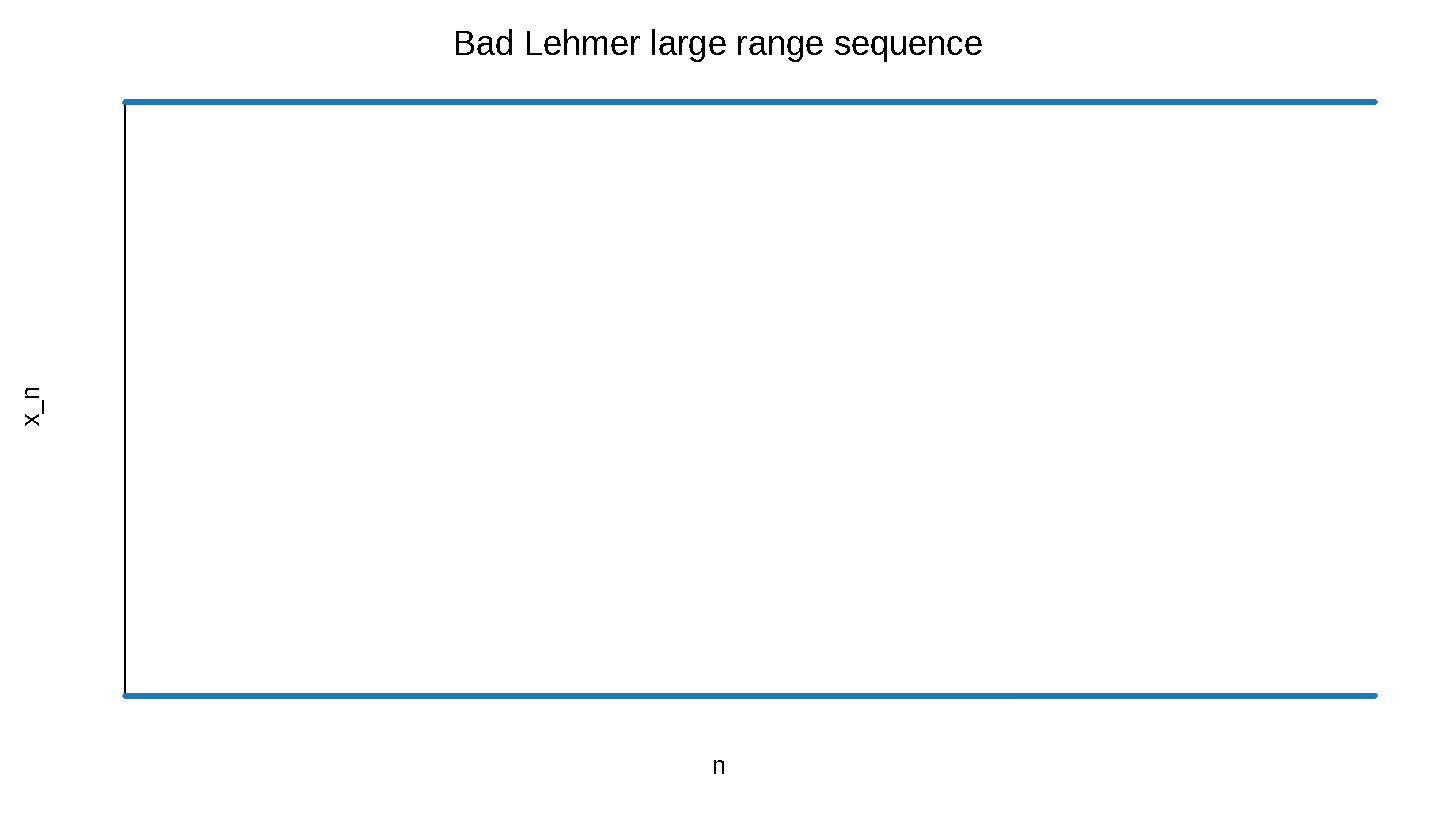
\includegraphics[width=0.48\textwidth]{figures/lehmer/bad_large_range/lehmer_bad_minus_one_multiplier_sequence.pdf}
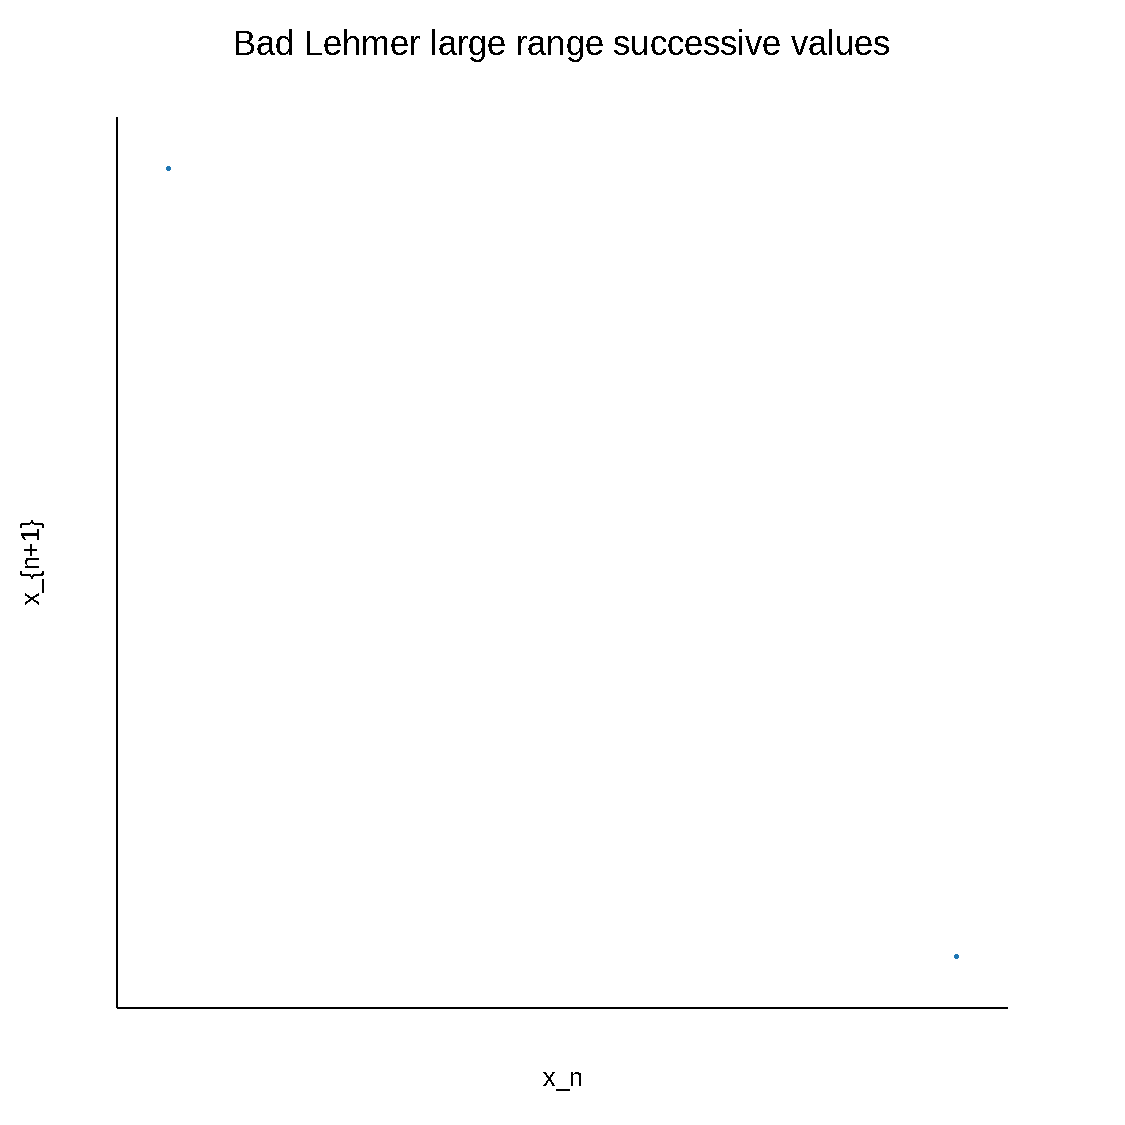
\includegraphics[width=0.48\textwidth]{figures/lehmer/bad_large_range/lehmer_bad_minus_one_multiplier_successive_values.pdf}
\caption{Sequence plot and successive-value plot for the bad large-range Lehmer generator}
\label{fig:lehmer-bad-seq-succ}
\end{figure}

Figures \ref{fig:lehmer-bad-hist-bits} and \ref{fig:lehmer-bad-seq-succ} show the weakness of choosing $a=m-1$. Although the numerical range looks large, the generator has period $2$ for a non-zero seed. The sequence plot alternates between two levels, and the successive-value plot collapses into a tiny set of points.

\begin{figure}[htbp]
\centering
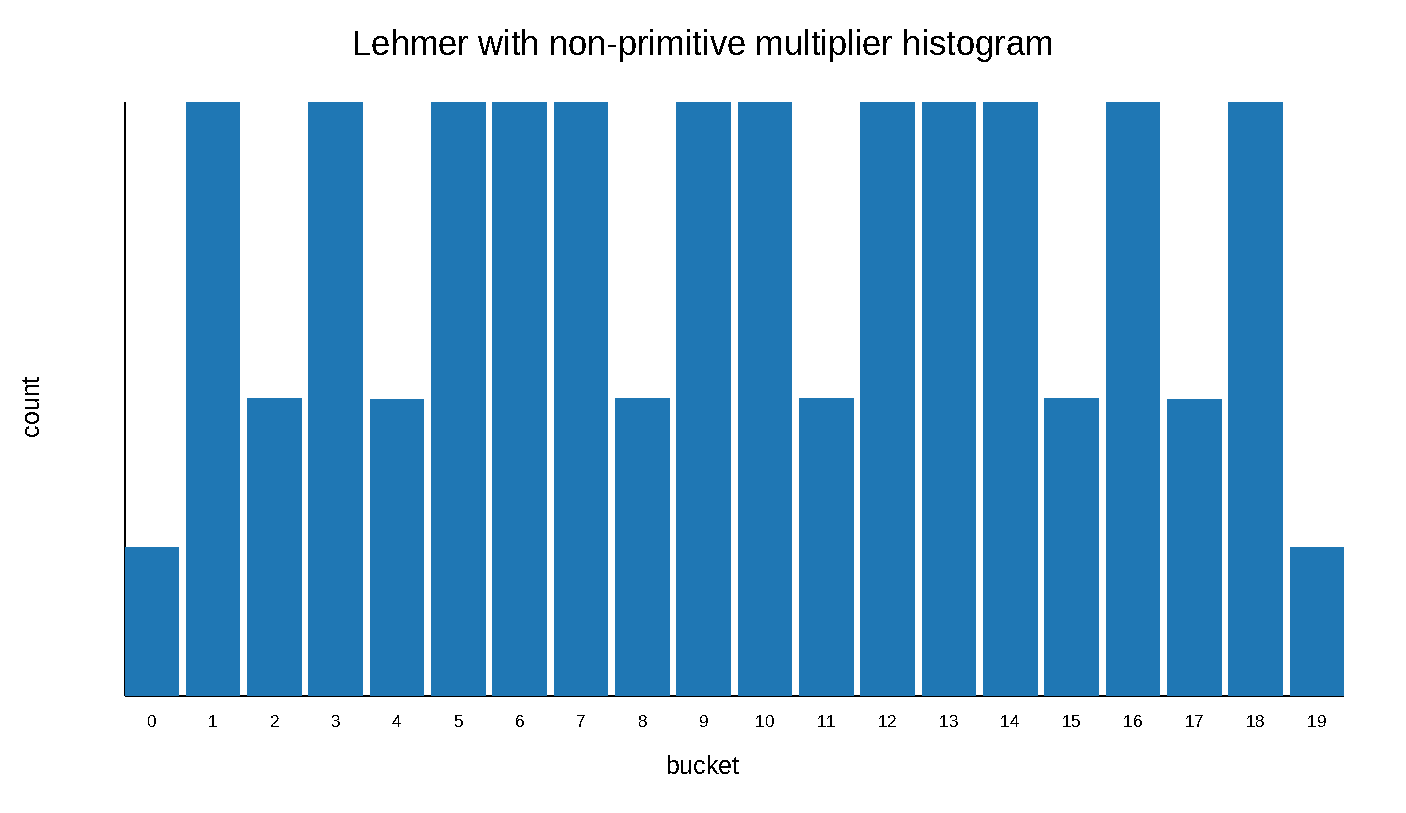
\includegraphics[width=0.48\textwidth]{figures/lehmer/single_bad_parameter/lehmer_single_bad_nonprimitive_multiplier_histogram.pdf}
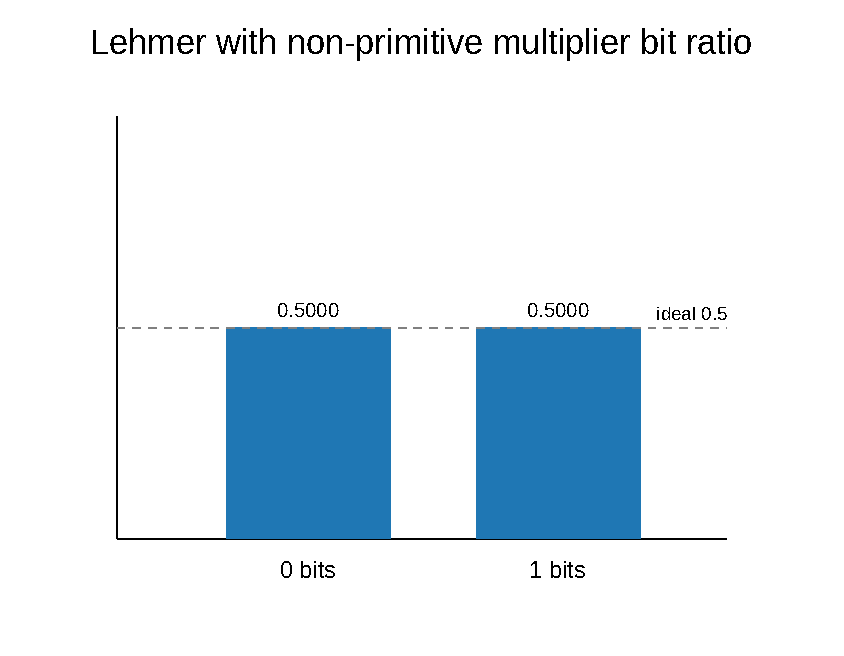
\includegraphics[width=0.48\textwidth]{figures/lehmer/single_bad_parameter/lehmer_single_bad_nonprimitive_multiplier_bit_ratio.pdf}
\caption{Histogram and bit ratio for the Lehmer generator with a non-primitive multiplier}
\label{fig:lehmer-single-hist-bits}
\end{figure}

\begin{figure}[htbp]
\centering
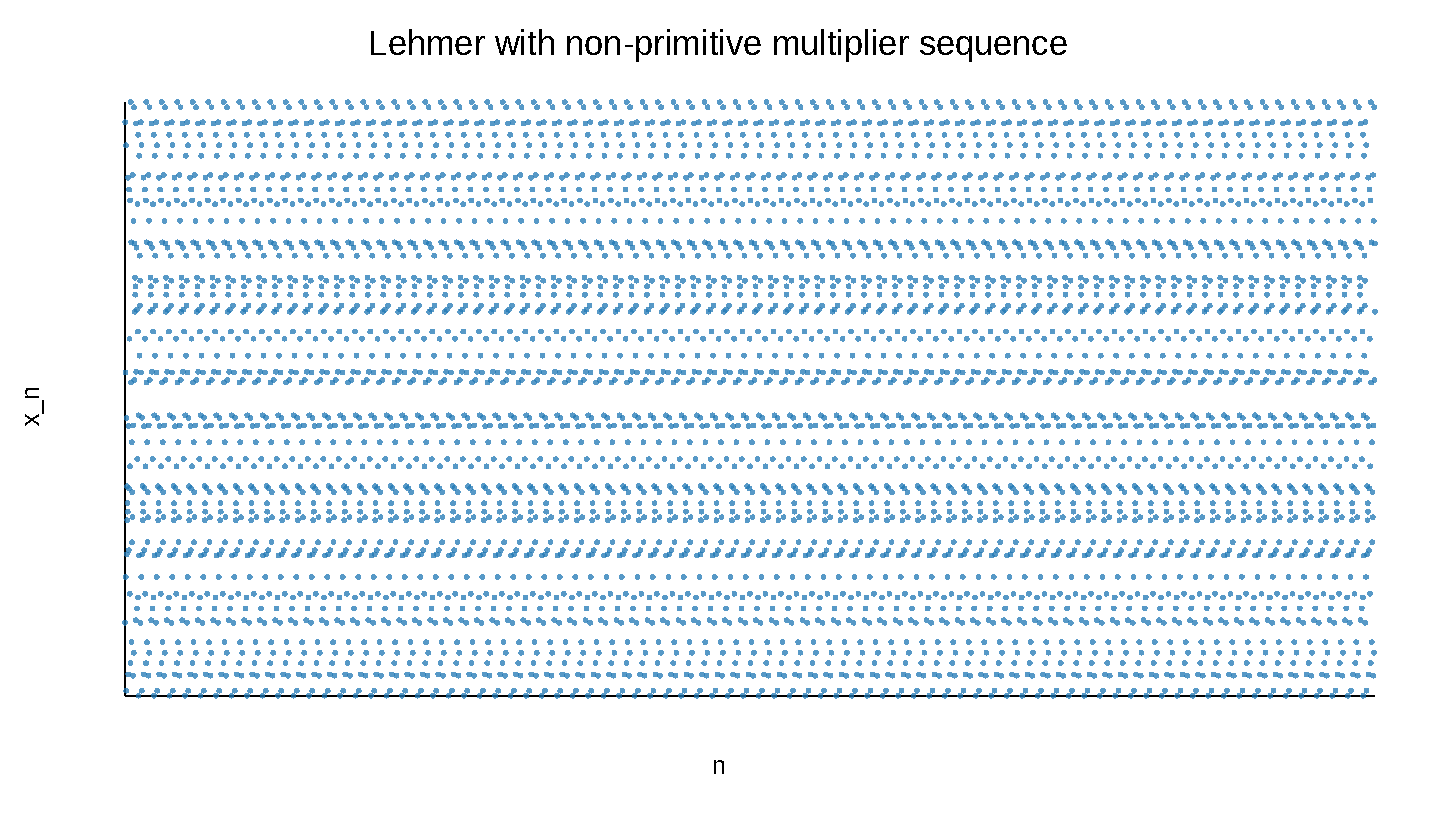
\includegraphics[width=0.48\textwidth]{figures/lehmer/single_bad_parameter/lehmer_single_bad_nonprimitive_multiplier_sequence.pdf}
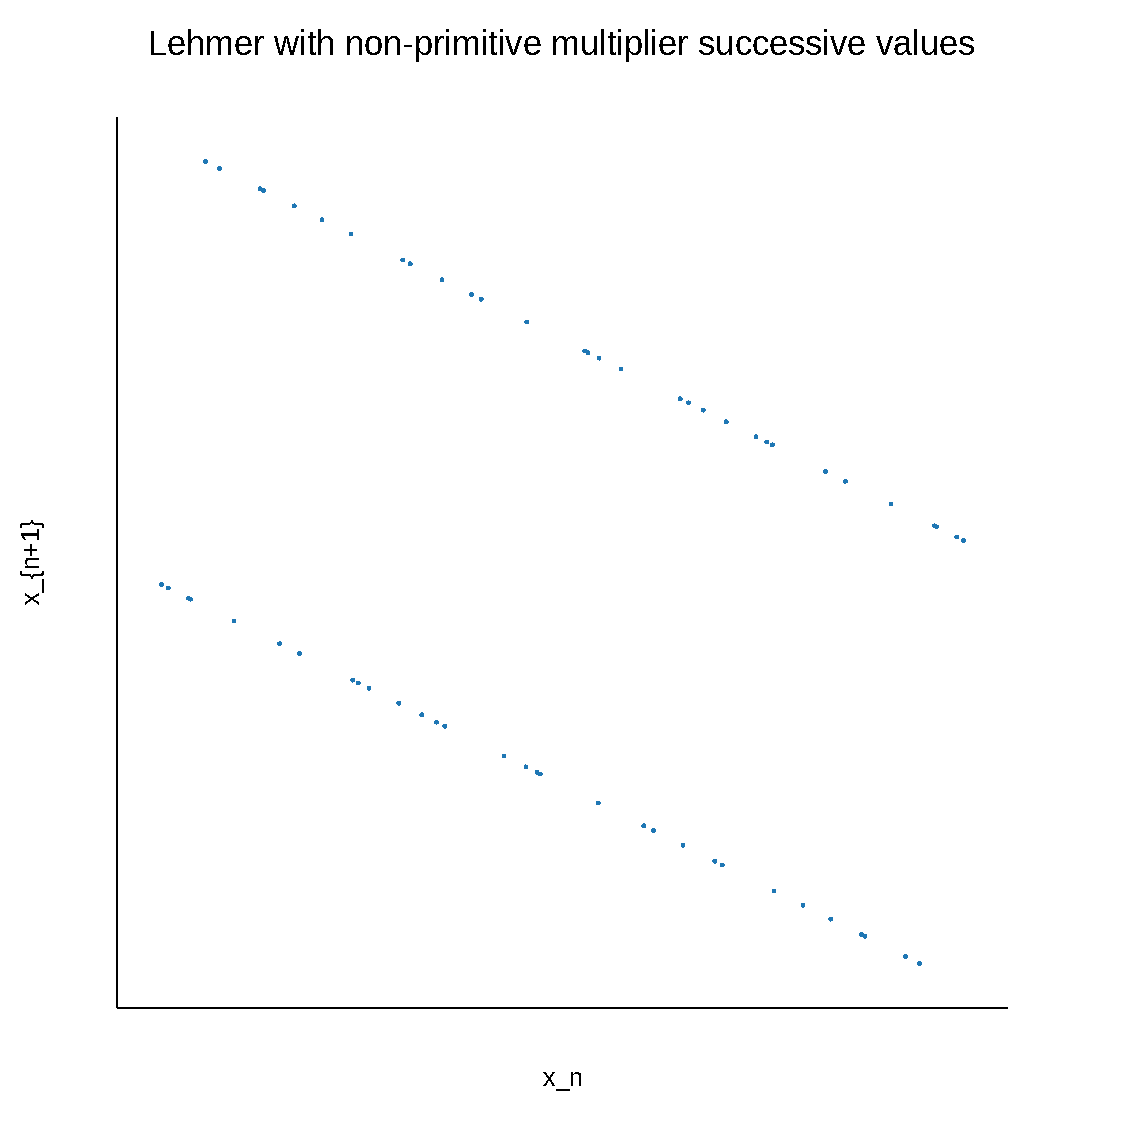
\includegraphics[width=0.48\textwidth]{figures/lehmer/single_bad_parameter/lehmer_single_bad_nonprimitive_multiplier_successive_values.pdf}
\caption{Sequence plot and successive-value plot for the Lehmer generator with a non-primitive multiplier}
\label{fig:lehmer-single-seq-succ}
\end{figure}

Figures \ref{fig:lehmer-single-hist-bits} and \ref{fig:lehmer-single-seq-succ} show a less trivial but still defective case. The generator is not stuck in a two-value cycle, but the histogram and chi-square value reveal that the distribution is far from the good variant. This demonstrates why the multiplier should be chosen carefully, preferably as a primitive root modulo the prime modulus.
\newpage
\subsection{Combined Generators}

Combined generators are constructed by combining multiple simpler generators in order to improve statistical properties and increase the effective period.

A typical construction is:

\[
x_n = (x_n^{(1)} - x_n^{(2)}) \bmod m,
\]

where $x_n^{(1)}$ and $x_n^{(2)}$ are independent sequences generated by two separate generators.

\subsubsection{Period}

If the individual generators have periods $T_1$ and $T_2$, then the period of the combined generator satisfies:

\[
T \mid \mathrm{lcm}(T_1, T_2),
\]

meaning that $T$ divides the least common multiple of the component periods.

\subsubsection{Advantages}

\begin{itemize}
    \item increased effective period,
    \item improved statistical behavior compared to single generators,
    \item reduced correlation between successive outputs.
\end{itemize}

\subsection{Summary}

Classical pseudorandom number generators such as LCG and Lehmer generators are simple and efficient but exhibit structural weaknesses, particularly in higher dimensions.

Combined generators partially address these issues by increasing period length and reducing correlation effects, but they still inherit linearity-based limitations.

These classical methods provide the foundation for understanding more advanced pseudorandom number generators introduced in later chapters.
